\chapter{Background}

This chapter will give insights into the most important topics and technologies relevant for this thesis. At the beginning, the 

Afterwards a brief overview of GraphQL is presented. Additional

\section{Micro-Frontend Architecture}

Micro-frontends try to apply the same principles from the microservice architecture to frontend development. Often times a microservice architecture with is developed by several teams has only one frontend application. Therefore, when adding new features a single team can be overwhelmed. Like a microservice architecture, a micro-frontend architecture focuses on developing many small frontend-applications, instead of developing a large software monolith. Each micro-frontend can be developed independently by another team. But a challenge is that the micro-frontend should appear as a single application to the user. Therefore, the different applications have to be integrated, which can be a challenge.

The term micro-frontend should not lead to false conclusions about the size of an application. The size of micro-frontends can vary. It can range from a simple login to a complex single-page application.

Building micro-frontends with the web allows different strategies of integrating the applications. Three different strategies exist to combine multiple micro-frontends into an app-shell. The client-side integration, the server-side integration and the combination of these two strategies and the combination of both strategies.



\subsection{Characteristics}

Micro-frontends tend to follow the same characteristics as microservices.

\subsubsection{Autonomous}

Technically a micro-frontend is a completely independent and runnable application.
The integration of the micro-frontends happens only through the frontend. The different micro-frontends are composed withing an app-shell. The application shell is a separete application that is usually the entry-point for the user to interact with all micro-frontends. The app-shell also provides the layout of the page and defines where the micro-frontends are placed.

\subsubsection{Technology Agnostic}

Just as microservices architectures, micro-frontend architectures can be technology agnostic. The current frontend development landscape offers a lot of JavaScript frameworks to choose from.

\subsubsection{Independently Depoyable}

The autonomy of micro-frontends offer the possibility for independent deployments. A large monolithical micro-frontends is trickier to deploy. There is no need to have communication over multiple teams to deploy the application.


\subsubsection{Small and Easy to Maintain}



\subsubsection{Resilience}



\subsubsection{Resilience}



\subsection{Integration strategies}

\subsubsection{Server-Side Integration}
\subsubsection{Client-Side Integration}

\subsection{Communication}

\subsection{Backend-For-Frontend Pattern}

\section{GraphQL}

The officical documentation states that GraphQL is a query language for APIs and a runtime for fulfilling those queries with your existing data. GraphQL provides a complete and understandable description of the data in your API, gives clients the power to ask for exactly what they need and nothing more, makes it easier to evolve APIs over time, and enables powerful developer tools. GraphQL is implemented in many languages and frameworks. It has a large ecosystem of libraries and tools.

\subsection{Origins and history}

GraphQL was initially developed at Facebook in 2012. In 2015 the project was made open-source and available to the public. The motivation behind the initial development of GraphQL was the limited flexibility of available API technologies like REST.

\subsection{Apollo Server and Client}

GraphQL is a query language and follows specific rules. The development of a GraphQL server and client is up to the application developer. Facebook has developed their own implementation of a GraphQL server and client. The server is called GraphQL.js and the client is called Relay.

Apollo 

Apollo Client is m

\subsubsection{How does the in-memory cache work?}

This section describes how the cache in apollo-client works. By default all GraphQL requests made with \textbf{ApolloClient} are cached inside the browsers memory. This enables Apollo Client to respond almost immediately to queries for already-cached data, without even sending a network request. This is needed, to ensure to reduce round-trips to the server in subsequent requests of the same query, because the requested data can be served from the cache. The caching mechanism reduces the load of the server, but introduces issues with cache management. \textbf{ApolloClient} includes a caching mechanism called ApolloCache and the propretary implementation called \textbf{InMemoryCache}. There are several Open-Source alternatives, that implement the \textbf{ApolloCache} interface.

\ifshowImages
\begin{figure}[!htbp]
\centering
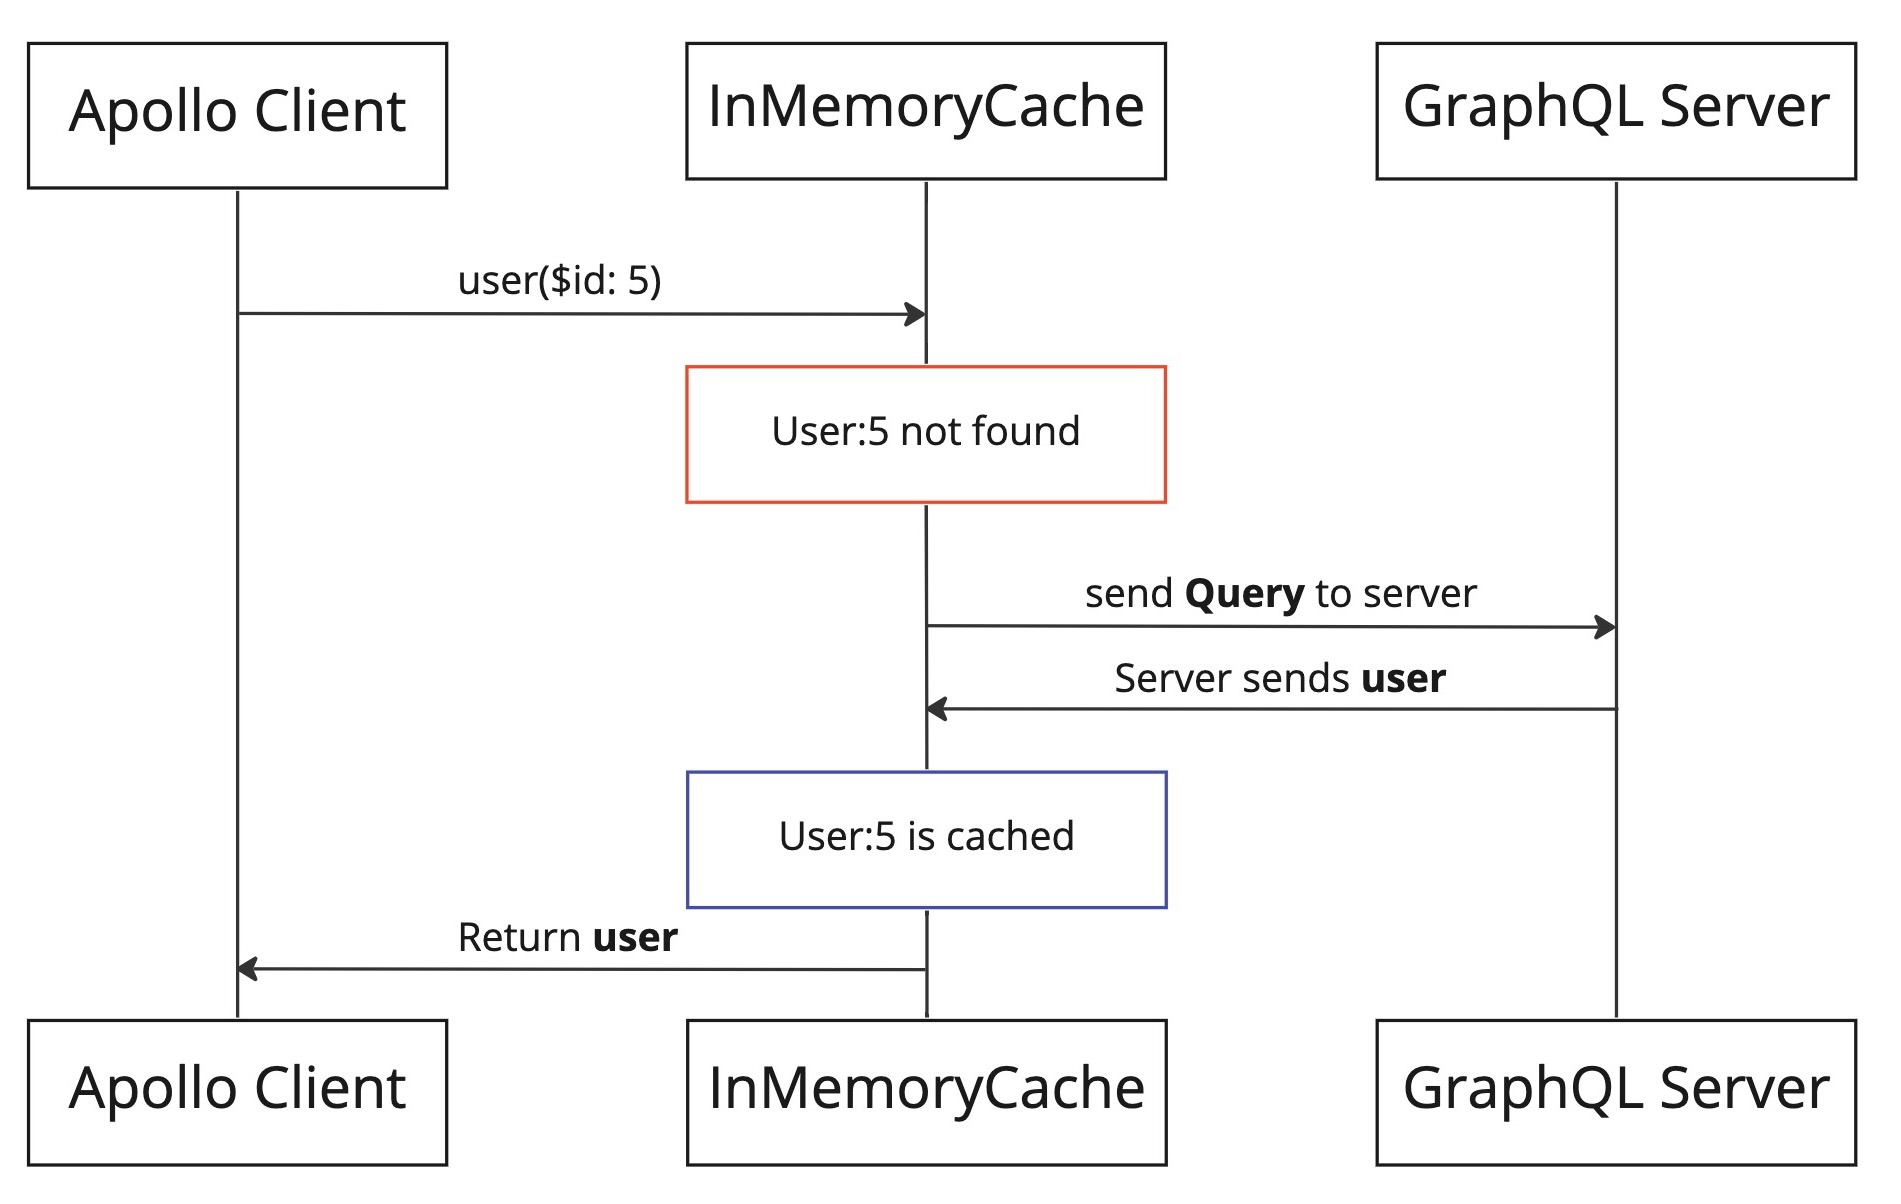
\includegraphics[width=0.6\linewidth]{images/background/apollo/apollo-client-basic-cache.jpeg}
\caption{All requests made during the measurement of the first approach}\label{figure:background:user-query-first-time}
\end{figure}
\fi

The flow of the cache, when the query \textbf{user} is executed the first time is shown in figure \ref{figure:background:user-query-first-time}.


\ifshowImages
\begin{figure}[!htbp]
\centering
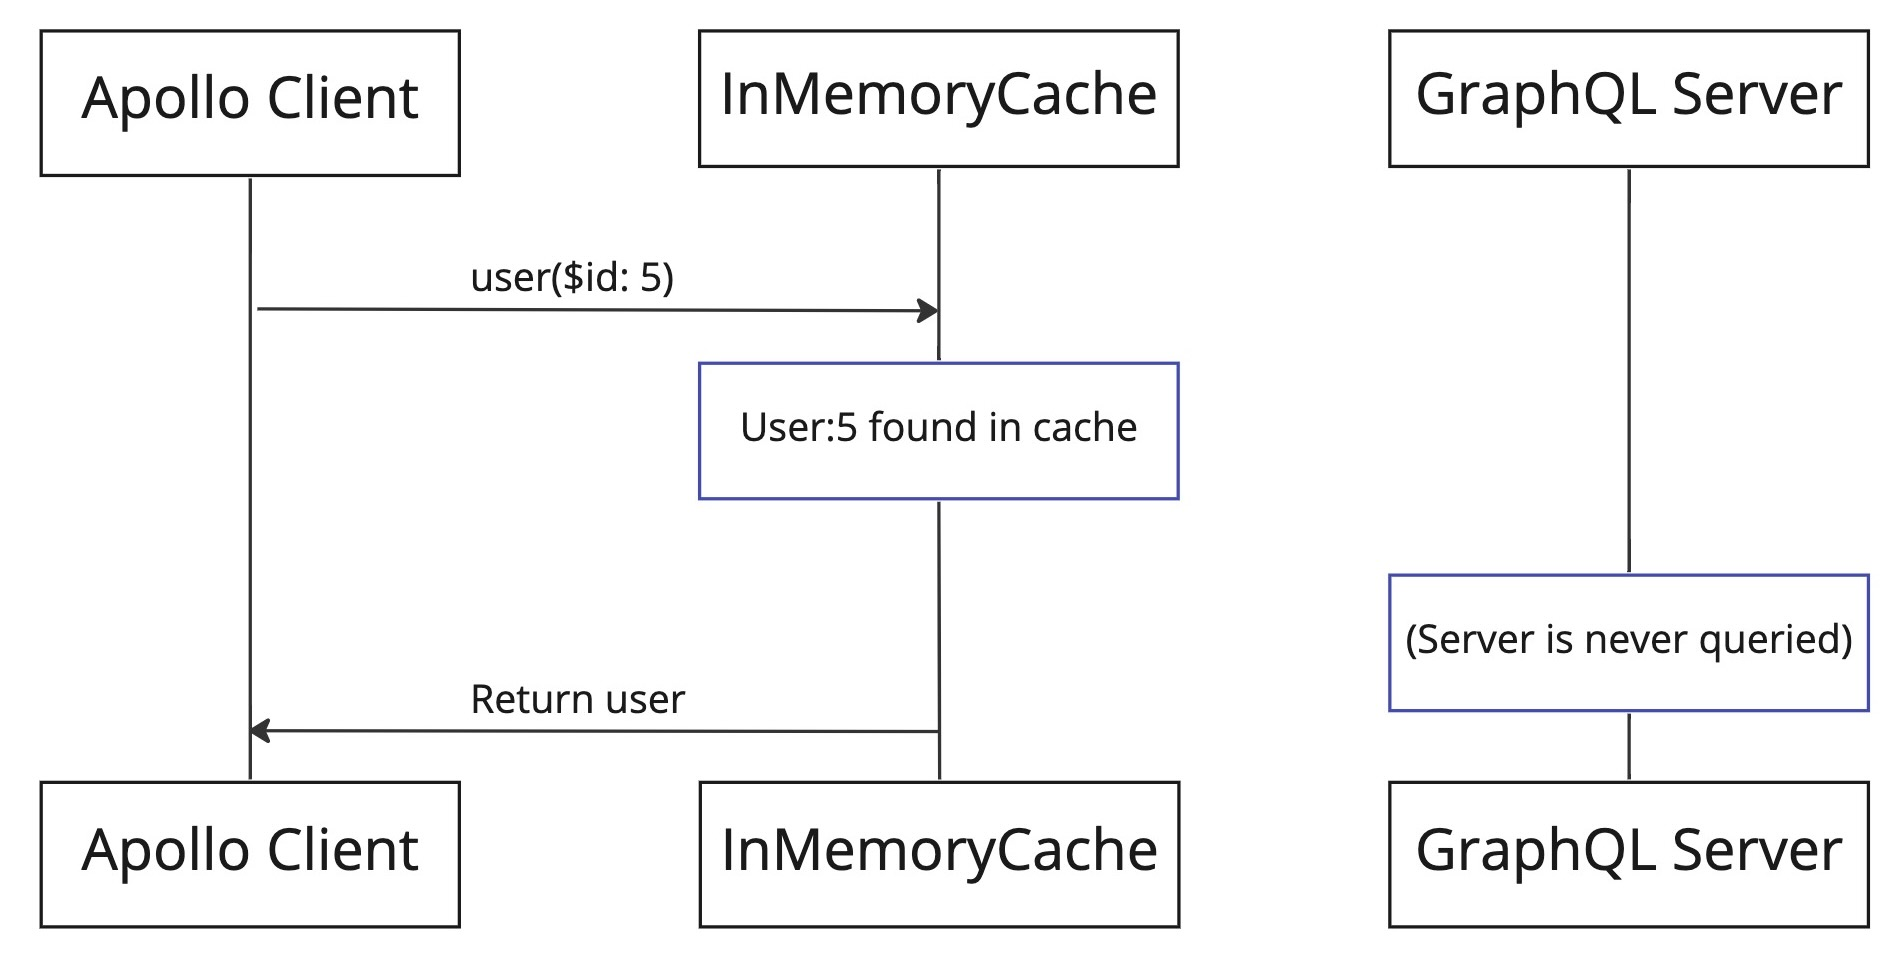
\includegraphics[width=0.6\linewidth]{images/background/apollo/apollo-client-basic-cache-warm.jpeg}
\caption{All requests made during the measurement of the first approach}\label{figure:background:user-query-second-time}
\end{figure}
\fi

When the query is executed later with the same parameters, the flow looks like in figure \ref{figure:background:user-query-second-time}.

In order to correctly understand cache updates, it is important to understand the structure of the cache. The structure of the \textbf{InMemoryCache} is a simple normalized object. When the cache is empty, it is just an empty object. When the following query is requested from the server and the response is stored in the cache, the cache will look like this:

\ifshowListings
\begin{listing}[H]
\begin{minted}{typescript}
query {
  users {
    id
    username
    email
  }
}
\end{minted}
\caption{An example of a query}\label{code:background:query-user-cache}
\end{listing}
\fi

And the server responds with the following result. The \textbf{\_\_typename} property is automatically appended to the query by the \textbf{ApolloClient}.

\ifshowListings
\begin{listing}[H]
\begin{minted}{typescript}
{
  users: [
    {
      __typename: 'User',
      id: '36bad921-8fcf-4f33-9f29-0d3cd70205c8',
      username: 'Florian',
      email: 'florian@test.io'
    }, 
    {
      __typename: 'User',
      id: 'a2096556-9a4e-4994-9de8-86c9e85ed6a1',
      username: 'Daniel',
      email: 'daniel@test.io'
    }
  ]
}
\end{minted}
\caption{The result of the GraphQL query from listing \ref{code:background:query-user-cache}}\label{code:background:query-user-response-result}
\end{listing}
\fi

The \textbf{ApolloClient} will update the cache so that it looks like this.

\ifshowListings
\begin{listing}[H]
\begin{minted}{typescript}
{
  ROOT_QUERY: {
    __typename: 'Query',
    users: [
      { __ref: 'User:36bad921-8fcf-4f33-9f29-0d3cd70205c8', },
      { __ref: 'User:a2096556-9a4e-4994-9de8-86c9e85ed6a1', },
    ],
  },
  'User:36bad921-8fcf-4f33-9f29-0d3cd70205c8': {
    __typeName: 'User',
    id: '36bad921-8fcf-4f33-9f29-0d3cd70205c8',
    username: 'Florian',
    email: 'florian@test.io',
  },
  'User:a2096556-9a4e-4994-9de8-86c9e85ed6a1': {
    __typeName: 'User',
    id: 'a2096556-9a4e-4994-9de8-86c9e85ed6a1',
    username: 'Daniel',
    email: 'daniel@test.io',
  }
}
\end{minted}
\caption{The data inside the cache with the response from listing \ref{code:background:query-user-response-result}}\label{code:background:query-user-cache-representation}
\end{listing}
\fi

Let's describe how the response from the server is transformed into the representation from the cache seen in listing \ref{code:background:query-user-cache-representation}. The cache object contains a key \textbf{ROOT\_QUERY}. This element contains the name of the queries that were executed and the results from all queries. The query \textbf{allUsers} was fetched, therefore the \textbf{ROOT\_QUERY} contains a field with the name \textbf{users}. The listing \ref{code:background:query-user-cache-representation} shows that the content of the \textbf{ApolloClient} is clearly different from the servers response. Instead of the user-information every array item consists of an object with a \textbf{\_\_ref} key. The value of the key is simply the \textbf{\_\_typename} and \textbf{id} of the user concatenated. The data from the response has been normalised and added to the cache object. Next to the \textbf{ROOT\_QUERY} element, the actual user-information is stored. Each has the same key as the \textbf{\_\_ref} from the \textbf{ROOT\_QUERY}. 

The same principle applies to arbitrary deep queries. The following query produces:

\ifshowListings
\begin{listing}[H]
\begin{minted}{typescript}
query {
  allUsers {
    id
    username
    Title {
      id
      name
    }
  }
}
\end{minted}
\caption{An example of a query}\label{code:background:nested-query-user-cache}
\end{listing}
\fi

And the server responds with the following result. The \textbf{\_\_typename} property is automatically appended to the query by the \textbf{ApolloClient}.

\ifshowListings
\begin{listing}[H]
\begin{minted}{typescript}
{
  users: [
    {
      __typename: 'User',
      id: '36bad921-8fcf-4f33-9f29-0d3cd70205c8',
      username: 'Florian',
      title: {
        __typename: 'Title',
        id: '2adb1120-d911-4196-ab1b-d5043cc7a00a',
        name: 'BSc.'
      }
    }, 
    {
      __typename: 'User',
      id: 'a2096556-9a4e-4994-9de8-86c9e85ed6a1',
      username: 'Daniel',
      title: {
        __typename: 'Title',
        id: '2adb1120-d911-4196-ab1b-d5043cc7a00a',
        name: 'BSc.'
      }
    }
  ]
}
\end{minted}
\caption{The result of the GraphQL query from listing \ref{code:background:nested-query-user-cache}}\label{code:background:nested-query-user-response-result}
\end{listing}
\fi

\ifshowListings
\begin{listing}[H]
\begin{minted}{typescript}
{
  ROOT_QUERY: {
    __typename: 'Query',
    users: [
      { __ref: 'User:36bad921-8fcf-4f33-9f29-0d3cd70205c8', },
      { __ref: 'User:a2096556-9a4e-4994-9de8-86c9e85ed6a1', },
    ],
  },
  'User:36bad921-8fcf-4f33-9f29-0d3cd70205c8': {
    __typeName: 'User',
    id: '36bad921-8fcf-4f33-9f29-0d3cd70205c8',
    username: 'Florian',
    Title: {
      __ref: 'Title:2adb1120-d911-4196-ab1b-d5043cc7a00a',
    },
  },
  'User:a2096556-9a4e-4994-9de8-86c9e85ed6a1': {
    __typeName: 'User',
    id: 'a2096556-9a4e-4994-9de8-86c9e85ed6a1',
    username: 'Daniel',
    Title: {
      __ref: 'Title:2adb1120-d911-4196-ab1b-d5043cc7a00a',
    },
  }
  'Title:2adb1120-d911-4196-ab1b-d5043cc7a00a': {
    __typeName: 'Address',
    id: '2adb1120-d911-4196-ab1b-d5043cc7a00a',
    name: 'BSc.',
  },
}
\end{minted}
\caption{The data inside the cache with the response from listing \ref{code:background:nested-query-user-response-result}}\label{code:background:nested-query-user-cache-representation}
\end{listing}
\fi

The \textbf{ROOT\_QUERY} is exactly the same as with the query before. Each user contains a reference to a title. Both users have the same title, therefore the server returned duplicate data. But the cache normalisation causes the title to be only present once in the cache.

This behaviour is very helpful, because when a cache item is updated, the entire cache object doesn't have to be traversed in search for the instance that has been changed. Only a single item has to updated.

The cache normalisation works when the query contains either a \textbf{\_id} or \textbf{id} field. Without an id the object can't be normalized. Here is an example:

\ifshowListings
\begin{listing}[H]
\begin{minted}{typescript}
query {
  allUsers {
    id
    username
    Title {
      name
    }
  }
}
\end{minted}
\caption{An example of a query}\label{code:background:no-id-query-user-cache}
\end{listing}
\fi

The response: 

\ifshowListings
\begin{listing}[H]
\begin{minted}{typescript}
{
  users: [
    {
      __typename: 'User',
      id: '36bad921-8fcf-4f33-9f29-0d3cd70205c8',
      username: 'Florian',
      title: {
        __typename: 'Title',
        name: 'BSc.'
      }
    }, 
    {
      __typename: 'User',
      id: 'a2096556-9a4e-4994-9de8-86c9e85ed6a1',
      username: 'Daniel',
      title: {
        __typename: 'Title',
        name: 'BSc.'
      }
    }
  ]
}
\end{minted}
\caption{The result of the GraphQL query from listing \ref{code:background:no-id-query-user-cache}}\label{code:background:no-id-query-user-response-result}
\end{listing}
\fi

And the cache looks like the following:

\ifshowListings
\begin{listing}[H]
\begin{minted}{typescript}
{
  ROOT_QUERY: {
    __typename: 'Query',
    users: [
      { __ref: 'User:36bad921-8fcf-4f33-9f29-0d3cd70205c8', },
      { __ref: 'User:a2096556-9a4e-4994-9de8-86c9e85ed6a1', },
    ],
  },
  'User:36bad921-8fcf-4f33-9f29-0d3cd70205c8': {
    __typeName: 'User',
    id: '36bad921-8fcf-4f33-9f29-0d3cd70205c8',
    username: 'Florian',
    Title: {
      name: 'BSc.',
    },
  },
  'User:a2096556-9a4e-4994-9de8-86c9e85ed6a1': {
    __typeName: 'User',
    id: 'a2096556-9a4e-4994-9de8-86c9e85ed6a1',
    username: 'Daniel',
    Title: {
      name: 'BSc.',
    },
  }
}
\end{minted}
\caption{The data inside the cache with the response from listing \ref{code:background:no-id-query-user-response-result}}\label{code:background:no-id-query-user-cache-representation}
\end{listing}
\fi

This should be avoided. If data of an unnormalized object has to be updated every occurrence of the item in the cache has to be updated manually. You must also never request the same thing sometimes with an id and sometimes without, because \textbf{ApolloClient} will throw an error when trying to update the cache after such a query.

The Apollo Client's cache stores the data a flat lookup table of objects that reference each other. These objects correspond to the objects that are returned by the GraphQL queries. A single cached object might include fields that were fetched by multiple queries. That means that multiple queries can fetch different fields for the same object. Before storing the data, the cache needs to normalize it. \cite{misc:-:apollo-cache-overview}

Whenever the Apollo Client receives the response data of a query it does the following. a

\paragraph{1. Identify objects} 

The cache identifies all distinct objects included in query response.

\begin{itemize}
  \item A \textbf{User} with id \textbf{36bad921-8fcf-4f33-9f29-0d3cd70205c8}
  \item A \textbf{User} with id \textbf{a2096556-9a4e-4994-9de8-86c9e85ed6a1}
\end{itemize}

\paragraph{2. Generate cache IDs} 

After identifying all objects, the cache generates a cache ID for each object. A cache ID uniquely identifies a particular object, while it is in the \textbf{InMemoryCache}.

So, the cache IDs for the objects are: 

\begin{itemize}
  \item \textbf{User:36bad921-8fcf-4f33-9f29-0d3cd70205c8}
  \item \textbf{User:a2096556-9a4e-4994-9de8-86c9e85ed6a1}
\end{itemize}

By default, an object's cache ID is the concentation of the object's \textbf{\_\_typename} and \textbf{id} (or \textbf{\_id}) fields.

If the cache can't generate a cache ID for a particular object, that object is directly cached inside its parent object, and must be referenced via the parent. Therefore the cache is not always completely flat.

\paragraph{3. Replace object fields with references} 

Next, the cache takes each field that contains an object and replaces its value with a reference to the appropriate object.

...

\paragraph{4. Store normalized objects} 

The resulting objects are stored inside the cache's flat lookup table. Whenever an incoming object has the same cache ID as an existing cached object, the fields of those objects are merged together. If the incoming and the existing object

